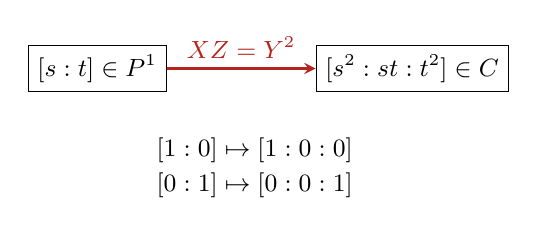
\begin{tikzpicture}[>=stealth,font=\small]
\node[draw] (a) at (0,0) {$[s:t]\in\mathbb P^1$};
\node[draw] (b) at (4,0) {$[s^2:st:t^2]\in C$};
\draw[->,BrickRed,thick] (a)--node[above] {$XZ=Y^2$}(b);
\node[below] at (2,-.75) {$[1:0]\mapsto[1:0:0]$};
\node[below] at (2,-1.2) {$[0:1]\mapsto[0:0:1]$};
\end{tikzpicture}
